\documentclass[12pt]{article}
%\usepackage{fullpage}
\usepackage{epic}
\usepackage{eepic}
\usepackage{paralist}
\usepackage{graphicx}
\usepackage{algorithm,algorithmic}
\usepackage{tikz}
\usepackage{xcolor,colortbl}
\usepackage{amsmath, amssymb}

%%%%%%%%%%%%%%%%%%%%%%%%%%%%%%%%%%%%%%%%%%%%%%%%%%%%%%%%%%%%%%%%
% This is FULLPAGE.STY by H.Partl, Version 2 as of 15 Dec 1988.
% Document Style Option to fill the paper just like Plain TeX.

\typeout{Style Option FULLPAGE Version 2 as of 15 Dec 1988}

\topmargin 0pt
\advance \topmargin by -\headheight
\advance \topmargin by -\headsep

\textheight 8.9in

\oddsidemargin 0pt
\evensidemargin \oddsidemargin
\marginparwidth 0.5in

\textwidth 6.5in
%%%%%%%%%%%%%%%%%%%%%%%%%%%%%%%%%%%%%%%%%%%%%%%%%%%%%%%%%%%%%%%%

\pagestyle{empty}
\setlength{\oddsidemargin}{0in}
\setlength{\topmargin}{-0.8in}
\setlength{\textwidth}{6.8in}
\setlength{\textheight}{9.5in}

\setcounter{secnumdepth}{0}

\setlength{\parindent}{0in}
\addtolength{\parskip}{0.2cm}
\setlength{\fboxrule}{.5mm}\setlength{\fboxsep}{1.2mm}
\newlength{\boxlength}\setlength{\boxlength}{\textwidth}
\addtolength{\boxlength}{-4mm}

\newcommand{\algosolutionbox}[2]{
  \begin{center}
    \framebox{\parbox{\boxlength}{
        \textbf{CS 5722, Fall 2014} \hfill \textbf{#1}\\
        #2
      }}
  \end{center}}

\begin{document}

\algosolutionbox{Homework 8}{
  % TODO: fill in your own name, netID, and collaborators
  Group: Michael Jalkio, Kevin Li, Daniel Sperling\\
  NetIDs: mrj77, kyl27, dhs252
}

\section{1}
\subsection{a}
See graph.

\subsection{b}
\subsubsection{i}
See graph.
\subsubsection{ii}
TODO.

Graph follows on the subsequent page.

\subsection{c}
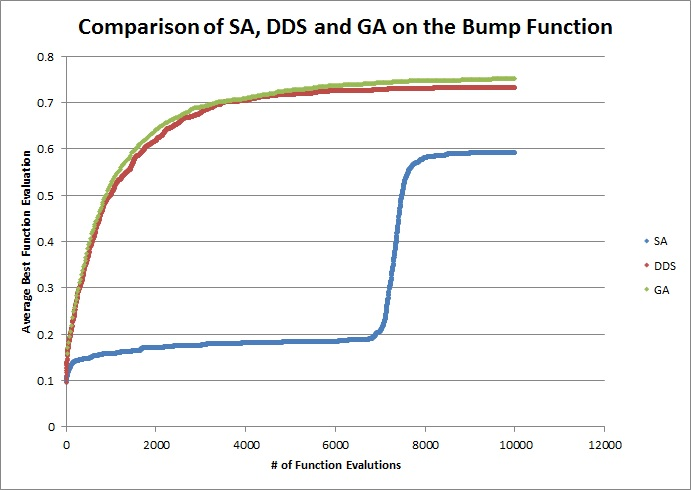
\includegraphics[scale=0.9]{abc_graph}

From the graph alone, it is clear that both GA and DDS dominate SA. It also appears that GA performs slightly better than DDS over the course of the run, and may dominate at the end.

\subsection{d}

\subsubsection{Comparison 1: Box Plot}
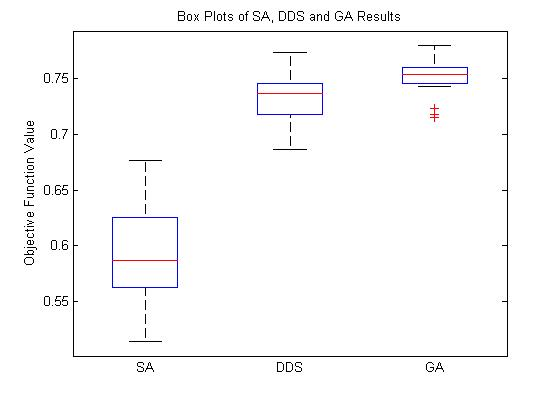
\includegraphics[scale=0.6]{boxplot}\\
\subsubsection{Comparison 2: CDF}
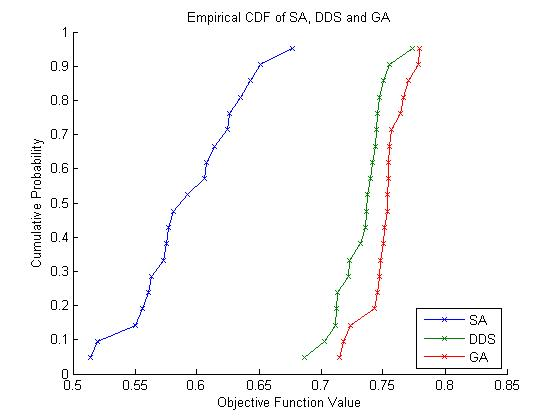
\includegraphics[scale=0.6]{cdf}\\

\subsubsection{Comparison 3: Two sample t test}

The null hypothesis for each pair is that the mean value of the two search heuristics is the same.\\\\

SA/DDS:\\\\
Statistics: T Statistic: -13.509848\\
P value for Two Sided: 0.00000\\
P value for One Sided: 0.000000\\

For comparison at $\alpha = 0.05$, $t_{\alpha/2,v} = 2.052042$, $t_{\alpha, v}  = 1.703421$. As $t < -t_{\alpha/2,v}$, we reject the null hypothesis and accept that the two mean values are different. Then, since $t <= -t_{\alpha, v}$, we can accept the alternate hypothesis that $\mu_x - \mu_y < \Delta_0$, indicating that the mean of SA is statistically significantly less than the mean of DDS.\\\\
As the means were so far off, it can easily be seen that SA performed much worse than DDS. This confirms what was seen in the graph in part c, the box plot above, and in the cdf, where DDS dominated SA.\\\\

SA/GA:\\\\
Statistics: T Statistic: -15.615549\\
P value for Two Sided: 0.000000\\
P value for One Sided: 0.000000\\

For comparison at $\alpha = 0.05$, $t_{\alpha/2,v} = 2.058272$, $t_{\alpha, v}  = 1.707344$. As $t < -t_{\alpha/2,v}$, we reject the null hypothesis and accept that the two mean values are different. Then, since $t <= -t_{\alpha, v}$, we can accept the alternate hypothesis that $\mu_x - \mu_y < \Delta_0$, indicating that the mean of SA is statistically significantly less than the mean of GA.\\\\
As the means were so far off, it can easily be seen that SA performed much worse than GA. This confirms what was seen in the graph in part c, the box plot above, and in the cdf, where GA dominated SA.\\\\

DDS/GA:\\\\
Statistics: T Statistic: -3.172571\\
P value for Two Sided: 0.003015\\
P value for One Sided: 0.001508\\

For comparison at $\alpha = 0.05$, $t_{\alpha/2,v} = 2.025410$, $t_{\alpha, v}  = 1.686598$. As $t < -t_{\alpha/2,v}$, we reject the null hypothesis and accept that the two mean values are different. Then, since $t <= -t_{\alpha, v}$, we can accept the alternate hypothesis that $\mu_x - \mu_y < \Delta_0$, indicating that the mean of SA is statistically significantly less than the mean of GA.\\\\
The means were significantly closer together in this pairing, but since both standard deviations were so low, it makes sense that we can still confirm that GA performed better than DDS. This confirms what was seen in the graph in part c, the box plot above, and in the cdf, where GA dominated DDS.

\section{2}
\subsection{a}
For a single iteration (a single generation) we can figure out the wall clock time.  We first have 50 seconds of serial calculations, then 10 seconds of communication, then each processor is able to handle the calculation of a single fitness function which takes 50 seconds, and finally we must perform communication again for 10 seconds.  For 100 generations we just need to multiply.  Therefore the total wall clock time is:
\begin{align*}
T(20) & = 100(50s + 10s + 50s + 10s)\\
& = 100 * 120s = 200m = 3hr \text{ and } 20m
\end{align*}
In serial the GA algorithm would take $100(50s + 20*50s)= 105000s = 1750m = 29 hr \text{ and } 10m$.  Therefore, the speedup is:
\begin{align*}
S(20) & = \frac{T(1)}{T(20)} = \frac{105000s}{12000s} = 8.75
\end{align*}
Which is fantastic!

\subsection{b}
Everything is exactly the same with 22 processors instead of 20.  Because there are only 20 offspring in each generation and we're not allowed to split the fitness calculation for one offspring between processors, we will always have 2 processors that are idle.

\subsection{c}
First we'll write speed up in terms of $T_F$:
\begin{align*}
S(20) & = \frac{100(50s + 20T_F)}{100(50s + 10s + T_F + 10s)}\\
& = \frac{50s + 20T_F}{70s + T_F}
\end{align*}
So efficiency with 20 processors is:
\begin{align*}
E(20) & = \frac{S(20)}{20} = \frac{50s + 20T_F}{20(70s + T_F)}
\end{align*}
And we can then solve for all values of $T_F$ which will lead to at least 80\% efficiency:
\begin{align*}
\frac{50s + 20T_F}{20(70s + T_F)} \ge 0.8\\
50s + 20T_F \ge 16(70s + T_F)\\
4T_F \ge 1070s\\
T_F \ge 267.5s
\end{align*}
Meanwhile efficiency for 22 processors is:
\begin{align*}
E(22) & = \frac{S(22)}{22} = \frac{50s + 20T_F}{22(70s + T_F)}
\end{align*}
And we can again solve for $T_F$ that leads to at least 80\% efficiency:
\begin{align*}
\frac{50s + 20T_F}{22(70s + T_F)} \ge 0.8\\
50s + 20T_F \ge 17.6(70s + T_F)\\
2.4T_F \ge 1182s\\
T_F \ge 492.5s
\end{align*}
The value of $T_F$ for 22 processors to be 80\% efficient is much higher than the value for 20 processors.  This is because 2 processors do no work at all and only serve to lower the efficiency compared to the 20 processor case.  We can imagine that each processor needs to handle a certain proportion of the speed up, but if 2 processors contribute none at all everything else needs to pick up the slack.  If we put the same $T_F=492.5s$ into the 20 processor case this actually leads to 88\% efficiency!

\end{document}